\section{Appendix}
\label{sec:app}

\subsection{Descriptive Statistics}

\begin{figure}[htbp]
    \centering
    \caption{Treatment status for the construction of a prison in a 300KM radius}
    \includegraphics[width=1\textwidth]{figures/descriptives/event_view_300KM.pdf}
    \label{fig:event_view_300km}
\end{figure}

% \begin{figure}[htb!]
% \small
%    \centering
%    \caption{Evolution of Monthly Registered Crimes in Mexico (2000-2010)}
%    \label{fig:figevo}
%    \includegraphics[width=.8\textwidth]{figures/descriptives/evolution.pdf}
%    \caption*{\footnotesize{This figure presents the trend of monthly registered crimes across Mexico from 2000 to 2012. The vertical red line represents the date where President Felipe Calderon took office (January 1st, 2006), while the vertical blue line represents the date where the Privatization contracts were signed \citep{Evalua}.}  \protect}
% \end{figure}

\input{tables/descriptives/statsprisons}

\subsection{Additional Mechanism Event Studies}

\begin{figure}[!htpb]
    \centering
    \caption{Dynamic effects of prison openings on arrests by type of crime}
    \label{fig:app_es_crime_type_all_1}
    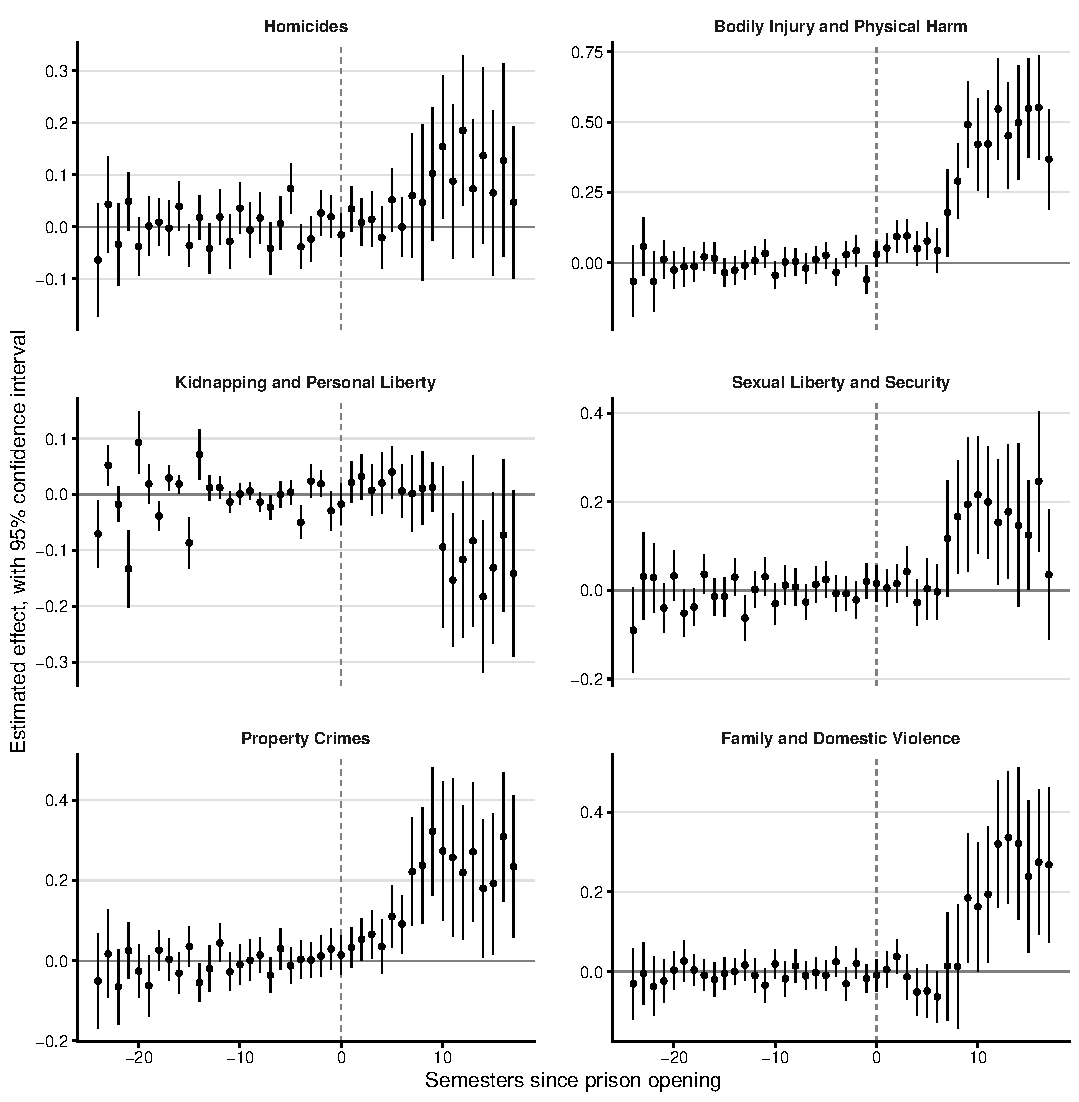
\includegraphics[width=\textwidth]{../../results/figures/final_paper/app_es_crime_type_all_1.pdf}
    \begin{minipage}{0.95\textwidth}
    \footnotesize \emph{Notes:} The figure reports CSDID event-study estimates with controls. Points denote dynamic treatment effects and vertical bars report 95 percent confidence intervals. Outcomes are crime-category arrest counts transformed using \(\log(1+y)\).
    \end{minipage}
\end{figure}

\begin{figure}[!htpb]
    \centering
    \caption{Dynamic effects of prison openings on arrests by type of crime}
    \label{fig:app_es_crime_type_all_2}
    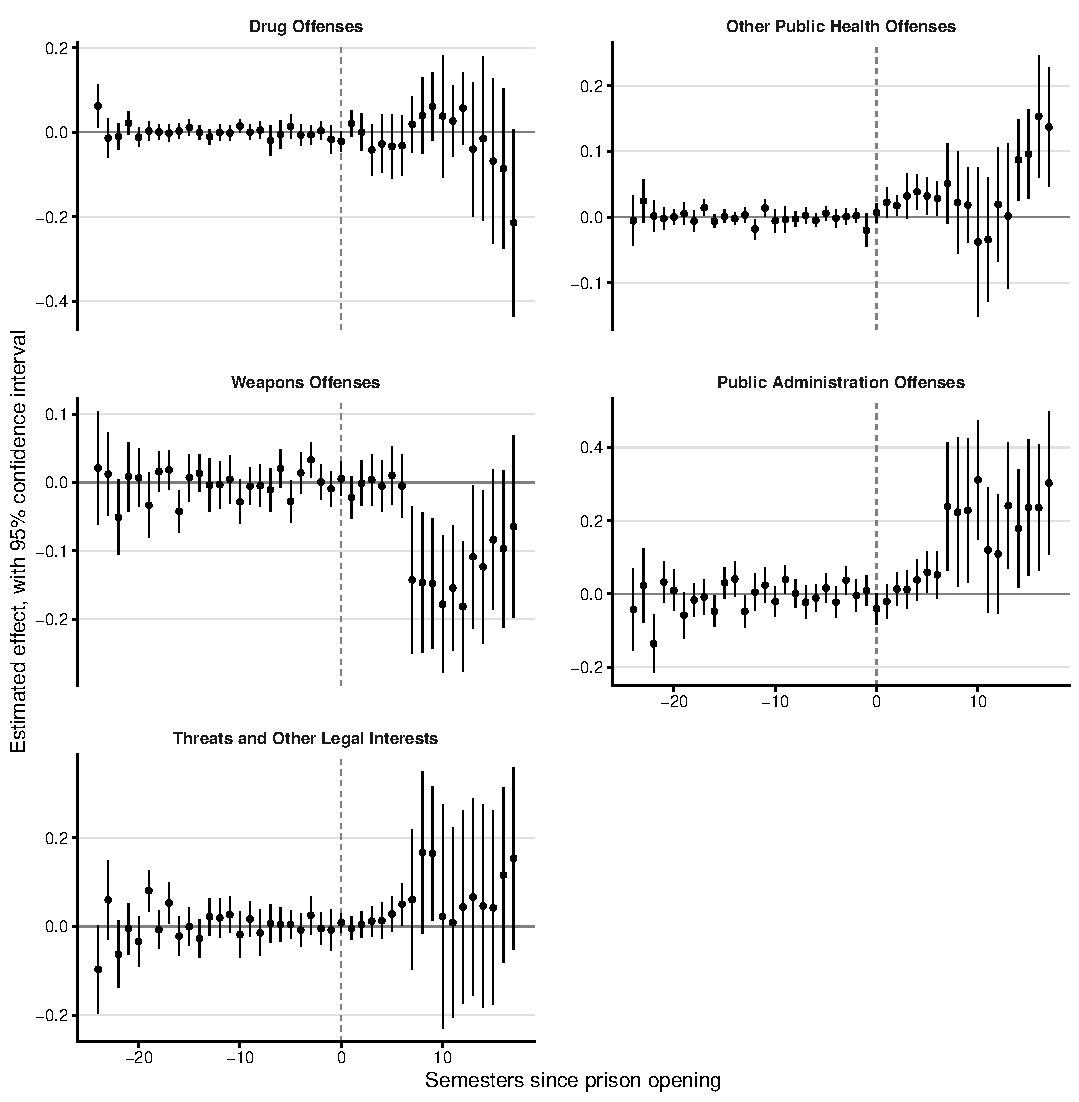
\includegraphics[width=\textwidth]{../../results/figures/final_paper/app_es_crime_type_all_2.pdf}
    \begin{minipage}{0.95\textwidth}
    \footnotesize \emph{Notes:} The figure reports CSDID event-study estimates with controls. Points denote dynamic treatment effects and vertical bars report 95 percent confidence intervals. Outcomes are crime-category arrest counts transformed using \(\log(1+y)\).
    \end{minipage}
\end{figure}



